\documentclass[14pt,a4paper]{article}

\usepackage[russian]{babel}
\usepackage{hyperref}
\usepackage{indentfirst}
\usepackage{float}
\usepackage{geometry}
\usepackage{graphicx}
\usepackage{verbatim}
\usepackage{wrapfig}

\setlength{\parindent}{0.5cm}
\geometry{top=2cm, bottom=2cm, left=1.5cm, right=1.5cm}
\renewcommand{\thesubsection}{\arabic{subsection}}
\renewcommand{\labelenumi}{\arabic{enumi})}  
\newcommand{\customtitle}[2]{%
\begin{titlepage}
  \begin{center}
    {\large\scshape\bfseries
    МИНИСТЕРСТВО НАУКИ И ВЫСШЕГО ОБРАЗОВАНИЯ РОССИЙСКОЙ ФЕДЕРАЦИИ\\
    ФЕДЕРАЛЬНОЕ ГОСУДАРСТВЕННОЕ АВТОНОМНОЕ ОБРАЗОВАТЕЛЬНОЕ УЧРЕЖДЕНИЕ ВЫСШЕГО
    ОБРАЗОВАНИЯ\\
    «СЕВЕРО-КАВКАЗСКИЙ ФЕДЕРАЛЬНЫЙ УНИВЕРСИТЕТ»\\
    ФАКУЛЬТЕТ МАТЕМАТИКИ И КОМПЬЮТЕРНЫХ НАУК ИМЕНИ ПРОФЕССОРА Н.И.ЧЕРВЯКОВА}
    \vfill
    \Large{\textbf{ЛАБОРАТОРНАЯ РАБОТА №#1}}\\[2mm]
    \large{Алгоритмизация и программирование}\\[6mm]
    \large{\textbf{#2}}\\[20mm]
  \end{center}
  \begin{flushright}
    \large{
      \textbf{Выполнил студент:}\\
      Сивко Иван Андреевич\\
      студент 2 курса\\
      группа ПМИ-б-о-23-2,\\
      направление подготовки 01.03.02\\[5mm]
      \textbf{Проверил:}\\
      Ассистент кафедры вычислительной\\
      математики и кибернетики, к.ф.-м.н.,\\
      Черкашина Анастасия Андреевна}
  \end{flushright}
  \vfill
  \centerline{ \the\year\ г. }
\end{titlepage}
    }

\newenvironment{fancyblock}
  {\large\bfseries\scshape}
  {}

\begin{document}
\customtitle{20}{Модули}
\large{\textbf{
\centerline{Вариант 9}
Цель:
}}
\begin{small}
\begin{itemize}
  \item Совершенствование навыков разработки программ в среде программирования MS Visual C++
  \item Совершенствование навыков в программировании с использованием модульного подхода
\end{itemize}
\end{small}
\section*{Задание 1}
\subsection{Условие:}
При наличии прототипа вызываемые функции не обязаны размещаться в одном файле с
вызывающей функцией. То есть, описание тел функций можно разместить в другом
файле, который необходимо подключить к исходному с использованием директивы
\texttt{\#include}.
Составить программу, содержащую обращение к функции вычисления максимума из
двух чисел:
Возможное решение данной задачи имеет вид:               
\begin{enumerate}
  \item Заголовочный файл \texttt{max.h}. Его текст:
    \begin{verbatim}
    #pragma once
    int max(int a, int b);
    \end{verbatim}
    Данный файл (\texttt{max.h}) добавляется в папку Файлы заголовков:
    \begin{figure}[H]
      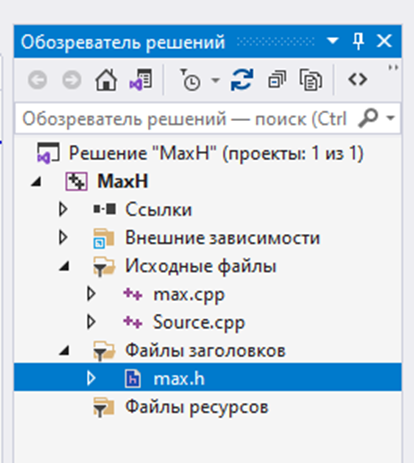
\includegraphics[width=0.3\textwidth]{data/condition20_1_1.png}
    \end{figure}
  \item Файл \texttt{source.cpp} содержит исходный код проекта:
    \begin{verbatim}
    /* включение заголовочного файла max.h, содержащего
       прототип функции max */
    #include <iostream>
    #include "max.h"
    
    using namespace std;
    
    int main() {
         int x, y, z;
         cout << "\n поочередно введите х и у \n";
         cin >> x >> y;
         z = max(x, y);       /* вызов функции */
         cout << "z=" << z;
         return 0;
    }
    \end{verbatim}
    \begin{minipage}{0.76\textwidth}
    \item Текст слева от картинки. Этот текст будет расположен в одном столбце. Вы
      можете продолжить писать текст, и он будет оставаться в этом столбце.
      Например, описание функции или другие комментарии.
    \begin{verbatim}
    int max (int a, int b) {
           int с;         //
           c=(a>b)?a:b;   //   тело функции 
           return с;      //              
    }
    \end{verbatim}
    \end{minipage}%
    \begin{minipage}{0.24\textwidth}
      \raggedleft
      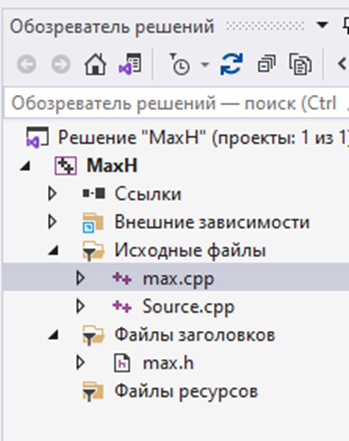
\includegraphics[width=0.90\textwidth]{data/condition20_1_2.png}  % Вставить изображение
    \end{minipage}
    Вызов функции является выражением в правой части оператора присваивания: 
    \begin{verbatim}
    z = max(x,y);
    \end{verbatim}
    при выполнении которого значения аргументов х и у подставляются вместо
    параметров а и b соответственно (передача параметров в функцию по
    значению). После выполнения тела функции возвращаемое значение передается в
    место вызова функции и присваивается переменной z. Описание функции
    находится в файле max.cpp, поэтому для включения файла в программу
    необходимо в тексте программы указать директиву препроцессора \#include
    "max.h".\\
    Описание функции может находиться в одном файле с главной программой. При
    этом директива \#include "max.h" не указывается, а вместо нее помещается
    описание функции.
\end{enumerate}
\subsection{Код + Результат работы программы:}
\begin{figure}[H]
  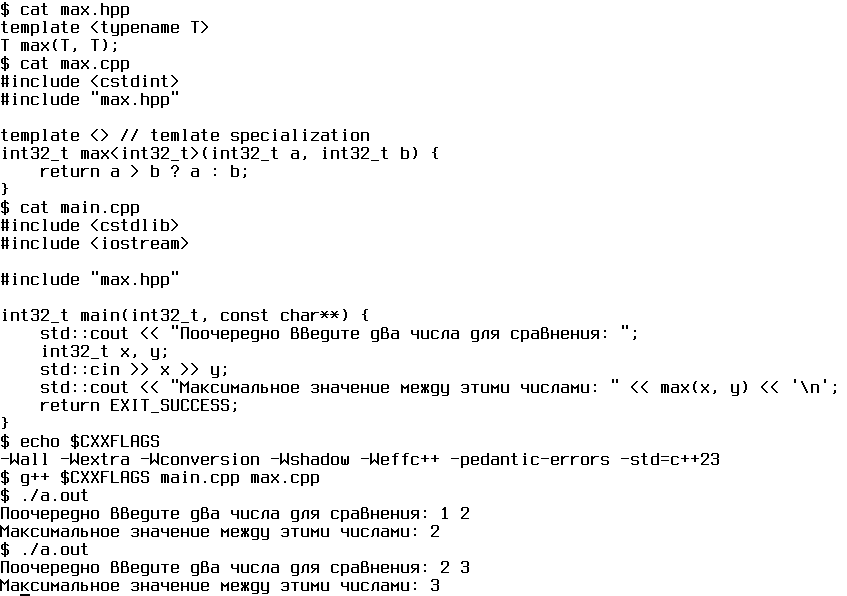
\includegraphics[width=0.7\textwidth]{data/demo20_1.png}
\end{figure}
\end{document}
